\documentclass[12pt,a4paper]{article}

\usepackage[utf8]{inputenc}
\usepackage[T1]{fontenc}
\usepackage[a4paper,margin=1in]{geometry}
\usepackage{lmodern}
\usepackage{microtype}
\usepackage{setspace}
\usepackage{booktabs}
\usepackage{longtable}
\usepackage{array}
\usepackage{graphicx}
\usepackage{xcolor}
\usepackage{hyperref}
\usepackage{enumitem}
\usepackage{listings}
\usepackage{amsmath}
\usepackage{tikz}
\usetikzlibrary{positioning,arrows.meta}

\hypersetup{
  colorlinks=true,
  linkcolor=blue,
  urlcolor=blue,
  pdftitle={Credit Risk AI v2.0 - Technical Report},
  pdfauthor={LoanVati Team}
}

\onehalfspacing
\setlength{\parindent}{0pt}
\setlength{\parskip}{0.5em}

\title{Credit Risk AI v2.0\\\large Technical Implementation Report}
\author{LoanVati Team}
\date{April 2026}

\begin{document}
\maketitle
\tableofcontents
\newpage

\section{Abstract}
This report documents the design and implementation of Credit Risk AI v2.0, a production-style decision support system for borrower risk assessment. The system combines traditional machine learning (Random Forest and Logistic Regression), SHAP-based model explanations, a FastAPI serving layer, and an agentic reporting pipeline (LangGraph + retrieval-augmented generation) integrated into a Streamlit user interface.

\section{Problem Statement and Objectives}
\subsection{Problem Statement}
Financial institutions need robust, explainable, and compliance-aware risk scoring workflows. Binary default prediction alone is often insufficient for operational lending decisions, especially in borderline cases requiring contextual explanation.

\subsection{Objectives}
\begin{itemize}[leftmargin=1.5em]
  \item Build an end-to-end borrower risk scoring pipeline.
  \item Provide reliable model performance with measurable recall and ROC-AUC.
  \item Surface explanation signals (top SHAP drivers) to support decision transparency.
  \item Generate structured lending reports grounded in retrieved regulatory context.
  \item Expose model and report workflows through API and interactive UI layers.
\end{itemize}

\section{System Architecture}
\subsection{High-Level Flow}
\begin{center}
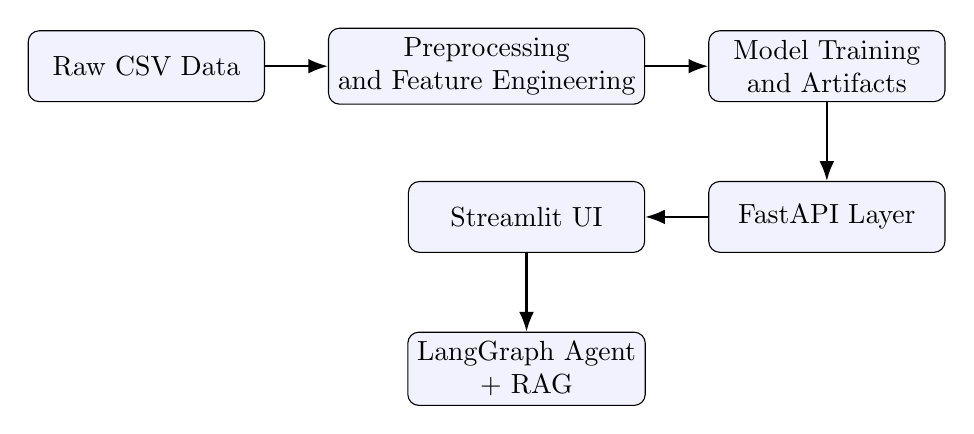
\begin{tikzpicture}[
  node distance=10mm and 8mm,
  box/.style={draw, rounded corners, align=center, minimum width=3.0cm, minimum height=0.9cm, fill=blue!5},
  arr/.style={-{Latex[length=2.5mm]}, thick}
]
\node[box] (raw) {Raw CSV Data};
\node[box, right=of raw] (prep) {Preprocessing\\and Feature Engineering};
\node[box, right=of prep] (train) {Model Training\\and Artifacts};
\node[box, below=of train] (api) {FastAPI Layer};
\node[box, left=of api] (ui) {Streamlit UI};
\node[box, below=of ui] (agent) {LangGraph Agent\\+ RAG};
\draw[arr] (raw) -- (prep);
\draw[arr] (prep) -- (train);
\draw[arr] (train) -- (api);
\draw[arr] (api) -- (ui);
\draw[arr] (ui) -- (agent);
\end{tikzpicture}
\end{center}

\subsection{Core Components}
\begin{itemize}[leftmargin=1.5em]
  \item \textbf{Preprocessing}: validation, joins/aggregations, engineered borrower-level features.
  \item \textbf{ML Modeling}: Random Forest and Logistic Regression with threshold tuning.
  \item \textbf{Explainability}: SHAP impact values and top contributing features per prediction.
  \item \textbf{Serving}: FastAPI endpoints for health, prediction, report generation, and preprocess trigger.
  \item \textbf{Agentic Reporting}: LangGraph node pipeline (Profile \textrightarrow{} Risk \textrightarrow{} Retrieval \textrightarrow{} Report).
  \item \textbf{UI}: Streamlit app with manual borrower input controls and results dashboard.
\end{itemize}

\section{Data and Feature Pipeline}
\subsection{Source Data}
The system is built around Home Credit style tabular sources. Raw files are mapped through dataset role names (application, bureau, previous applications, installments, card balances, POS cash, and metadata files).

\subsection{Preprocessing Steps}
\begin{enumerate}[leftmargin=1.7em]
  \item Validate file availability and schema constraints.
  \item Build aggregated borrower-level views from relational tables.
  \item Engineer ratio and behavior features (e.g., income and credit proportions).
  \item Save processed matrix to parquet for reproducible training.
\end{enumerate}

\section{Modeling and Evaluation}
\subsection{Model Family}
Two supervised learners are trained and evaluated:
\begin{itemize}[leftmargin=1.5em]
  \item Random Forest (primary inference model)
  \item Logistic Regression (benchmark baseline)
\end{itemize}

\subsection{Evaluation Metrics}
\begin{table}[h]
\centering
\begin{tabular}{lccc}
\toprule
Model & Recall & ROC-AUC & F1 \\
\midrule
Random Forest & 0.7126 & 0.7415 & 0.2502 \\
Logistic Regression & 0.7200 & 0.7501 & 0.2527 \\
\bottomrule
\end{tabular}
\caption{Reported model metrics from persisted evaluation artifacts.}
\end{table}

\subsection{Decision Thresholding}
Rather than using a fixed 0.5 threshold, the pipeline selects a threshold constrained by false positive rate limits, then applies business-oriented risk classes:
\begin{itemize}[leftmargin=1.5em]
  \item Low, Medium, High risk classes for typical probability bands.
  \item Manual review flag for borderline cases near decision threshold.
\end{itemize}

\section{Explainability and Agentic Reporting}
\subsection{Model Explainability}
Each prediction includes top feature contributions using SHAP values, enabling users to understand whether factors increase or decrease risk.

\subsection{Agent Workflow}
The agent pipeline follows four deterministic nodes:
\begin{enumerate}[leftmargin=1.7em]
  \item Profile analysis from borrower input.
  \item Risk reasoning from model outputs and SHAP signals.
  \item Regulatory retrieval from local vector index.
  \item Structured report generation with citations and disclaimer.
\end{enumerate}

\subsection{Structured Report Contract}
The final report contains five sections:
\begin{itemize}[leftmargin=1.5em]
  \item Profile
  \item Risk analysis
  \item Decision (APPROVE / REJECT / MANUAL REVIEW)
  \item Sources
  \item Disclaimer
\end{itemize}

\section{API and UI Implementation}
\subsection{FastAPI Endpoints}
The backend exposes operational endpoints for:
\begin{itemize}[leftmargin=1.5em]
  \item Health checks
  \item Prediction
  \item Agentic report generation
  \item Preprocessing refresh
  \item Metrics and threshold inspection
\end{itemize}

\subsection{Streamlit Frontend}
The frontend provides two workflows:
\begin{itemize}[leftmargin=1.5em]
  \item ML risk scoring dashboard with gauge, confidence, and ROC/confusion charts.
  \item AI lending report tab with step-by-step node progress and sourced output.
\end{itemize}

The latest interaction model uses manual form controls (sliders and textboxes) for borrower input in both tabs.

\section{Testing and Reliability}
The codebase includes tests for preprocessing logic, model behavior, API endpoints, RAG functionality, and report structure rules. Recent UI hardening includes graceful handling when model artifact files are missing, with user-facing instructions instead of application crashes.

\section{Primary Technology Stack}
\begin{longtable}{>{\raggedright\arraybackslash}p{0.35\textwidth}p{0.58\textwidth}}
\toprule
Category & Technologies \\
\midrule
Core Language & Python \\
ML and Data & scikit-learn, pandas, numpy, SHAP \\
Serving Layer & FastAPI, Uvicorn \\
Agent and RAG & LangGraph, LangChain, FAISS (vector index), sentence-transformers \\
LLM Integration & Groq API via LangChain connector \\
User Interface & Streamlit \\
Visualization & Plotly, Matplotlib \\
Documentation and SCM & LaTeX, GitHub \\
\bottomrule
\end{longtable}

\section{Limitations and Future Work}
\subsection{Current Limitations}
\begin{itemize}[leftmargin=1.5em]
  \item Model artifact generation depends on successful preprocessing and training runs.
  \item Local environment differences (compiler/toolchain) can affect optional dependencies.
  \item Dataset path consistency requires careful raw directory setup.
\end{itemize}

\subsection{Future Work}
\begin{itemize}[leftmargin=1.5em]
  \item Add robust environment checks and one-click setup scripts.
  \item Extend calibration and fairness diagnostics.
  \item Add batch scoring and downloadable report exports.
  \item Integrate CI workflows for automated training artifact validation.
\end{itemize}

\section{Responsible AI Statement}
This system is an AI-assisted decision support tool. It must not be used as the sole basis for adverse lending decisions. Human review, policy governance, and regulatory compliance checks are required before production decisioning.

\section{Conclusion}
Credit Risk AI v2.0 demonstrates a practical fusion of machine learning risk scoring and agentic regulatory reasoning. The implementation is modular, testable, and deployment-oriented, while preserving transparency through SHAP explanations and structured report outputs.

\end{document}
